% Source : http://forum.mathematex.net/latex-f6/repere-quelconque-en-tikz-t11475.html

\documentclass[10pt,a4paper]{article}
	\usepackage[utf8x]{inputenc}
	\usepackage{pgfplots}


\begin{document}

\section*{Méthode n°1}

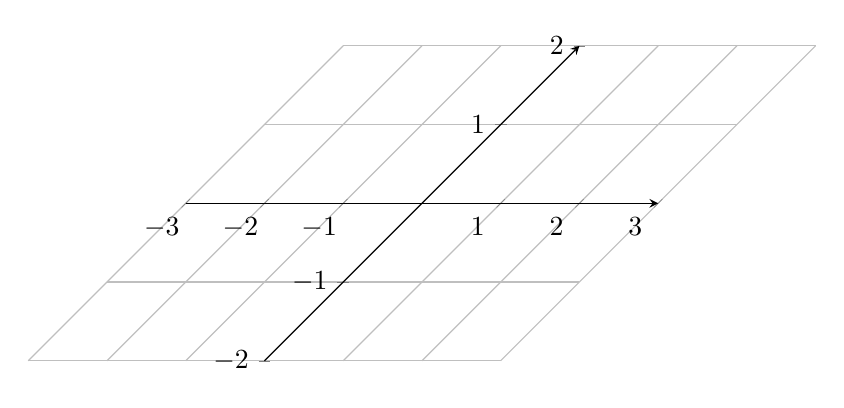
\begin{tikzpicture}
	\begin{axis}[axis lines=middle, grid=both,xtick={-3,-2,...,3},ytick={-2,-1,...,2},x=1cm,y={(1cm,1.0cm)},ymin=-2,ymax=2,xmin=-3,xmax=3]
	\end{axis}
\end{tikzpicture}


\section*{Méthode n°2}

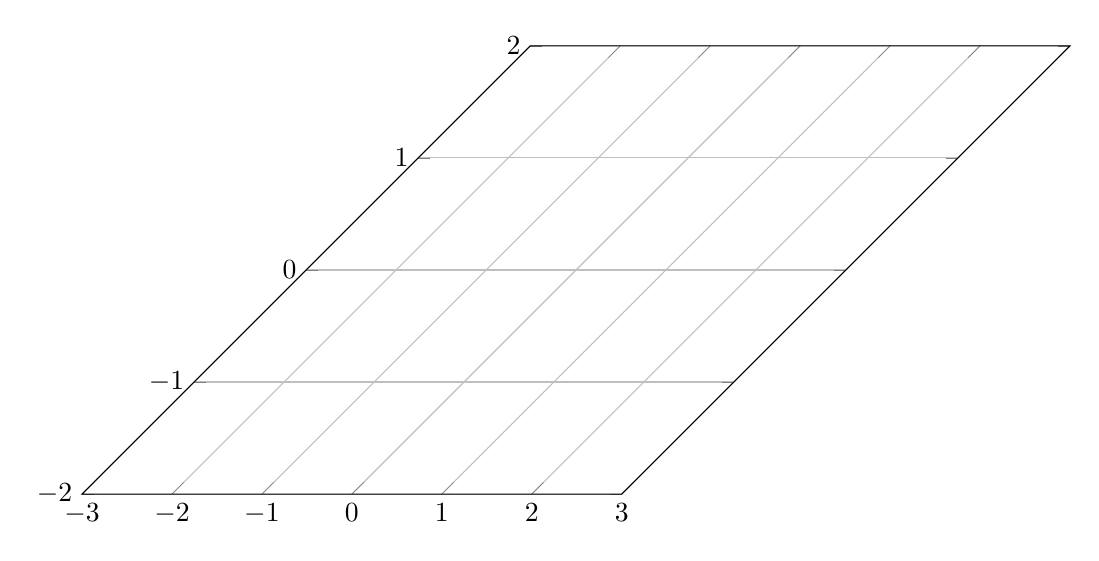
\begin{tikzpicture}[]
	\begin{axis}[xslant=1,grid=both,xtick={-3,-2,...,3},ytick={-2,-1,...,2},ymin=-2,ymax=2,xmin=-3,xmax=3]
	\end{axis}
\end{tikzpicture}


\section*{Méthode n°3}

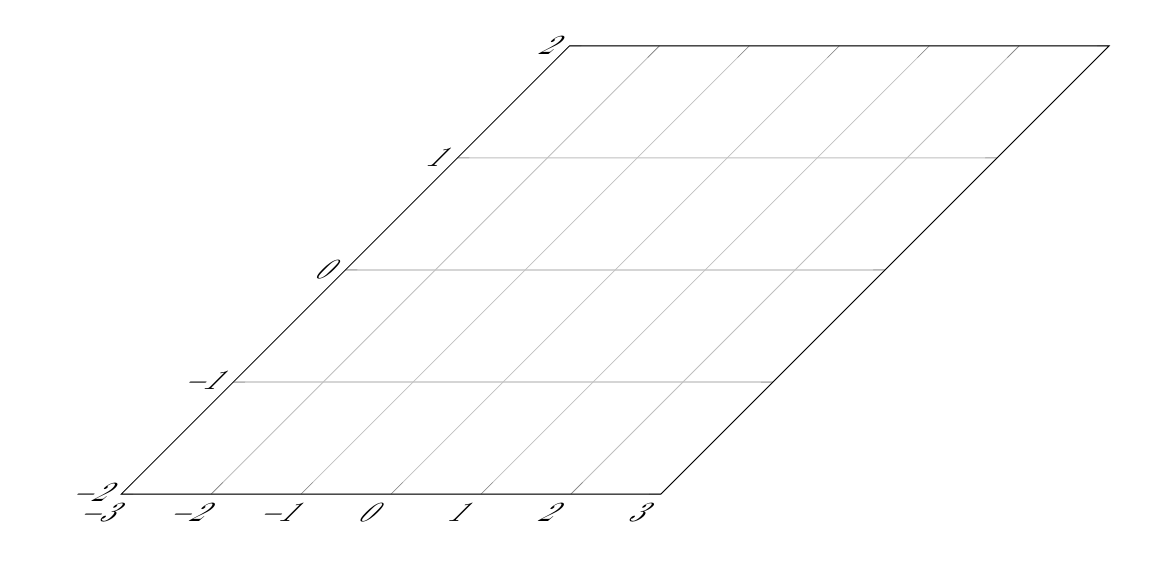
\begin{tikzpicture}[xslant=1]
	\begin{axis}[grid=both,xtick={-3,-2,...,3},ytick={-2,-1,...,2},ymin=-2,ymax=2,xmin=-3,xmax=3]
	\end{axis}
\end{tikzpicture}

\end{document}
